\chapter{Аналитическая часть}
\label{cha:analysis}
\section{Автоматическая обработка изображений человеческого лица}

В данной главе производится описание существующих исследований и технических аспектов, которые используются при автоматической обработке изображений человеческих лиц.


Связь подсистемы автоматической обработки человеческих лиц с другими подсистемами представлена на рисунке \ref{fig:sstructure}. Обобщенная процедура автоматического анализа человеческого лиц апредставлена на рисунке \ref{fig:face-analyse-structure}



Из рисунка \ref{fig:sstructure} видно, что управляющий модуль контролирует работу всей системы с помощью выдачи команд другим модулям.
Модуль получения изображений предоставляет изображения, например,  захватывая их с видеокамер, и управляющая программа может выводить результат пользователю.
Компонент автоматической обработки изображений для выделения человеческих лиц осуществляет обработку входных изображений и предоставляет результаты управляющему модулю.
Результатами могут являться:

\begin{enumerate}
  \item количество и позиции обнаруженных лиц;
  \item описание выражений обнаруженных лиц;
  \item гендерная классификация обнаруженных лиц;
  \item идентификация обнаруженных лиц.
\end{enumerate}


Модулю, предоставляющему изображения, могут посылать команды как управляющий так и анализирующий модули. Также в системах компьютерного зрения могут присутствовать и другие модули такие как:

\begin{enumerate}
  \item модуль распознавания речи;
  \item отслеживания перемещений объектов.
\end{enumerate}

Данные модули взаимодействуют с анализирующим модулем и производят дополнительную обработку для наделения обнаруженных объектов дополнительными свойствами, которые впоследствии отсылаются управляющей программе. Дополнительная информация об объекте может быть использована управляющей программой для более точного решения поставленных задач. Например, процедура идентификации человека может быть основана на информации о лице человека и его речи.


\begin{figure}
  \centering
  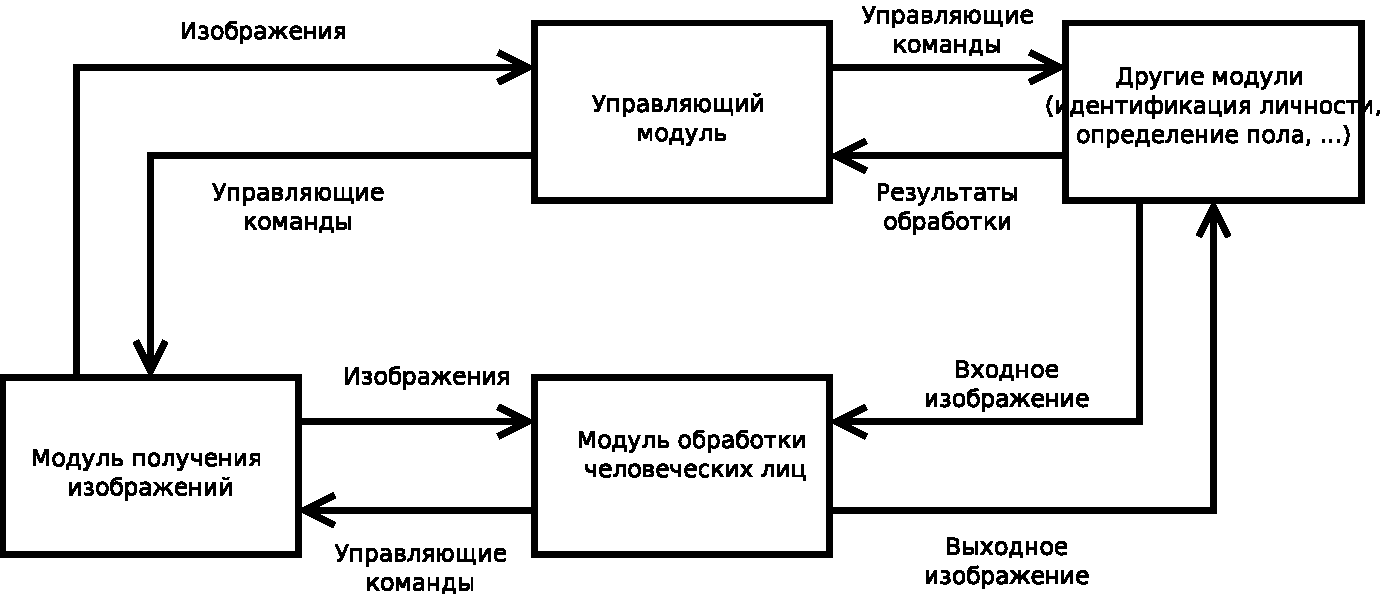
\includegraphics[width=\textwidth]{inc/dia/face-analyse-relation}
  \caption{Обобщенная структура модулей в системе распознавания человеческих лиц}
  \label{fig:sstructure}
\end{figure}

\begin{figure}
  \centering
  
\includegraphics[width=\textwidth]{inc/dia/face-analyse}
  \caption{Обобщенная структура модулей в системе распознавания человеческих лиц}
  \label{fig:face-analyse-structure}
\end{figure}


На рисунке \ref{fig:face-analyse-structure} показаны общие этапы процедуры автоматической обработки человеческих лиц на изображениях. Первым этапом процедуры является его локализация человеческого лица. В зависимости от целей приложения объект лица может отслеживаться на некоторой последовательности кадров, а может опеределяться обработкой одиночного изображения. Целью автоматической обработки человеческого лица является определение присутствия на входном изображении какого-либо количества человеческих лиц и их локализация. Отслеживание человеческого лица (tracking) означает определение траектории движения целевого объекта на последовательности кадров видеопотока. Выделение особенностей человеческого лица означает определение по изображению лица расположение глаз, носа, рта и других частей лица, в зависимости от решаемой задачи. Результаты первого этапа могут использоваться в первоначальном виде, однако в большинстве случаев применяют процедуру нормализации. Целью является снижение влияния на изображение различного освещения. Нормализованное изображение может подвергаться процедуре классификации. Однако осуществляется подготовительный этап --- составления входного вектора для классификатора. В простейшем случае таким ветором может являться последовательный набор пикселей исследуемого изображения.

Этап классификации может решать несколько задач. Например, определение пола, возраста, рассовой принадлежности, эмоций. Задачи могут решаться полностью самостоятельно, но иногда более выгодно последовательное решение задач. Так, например, если задачи определения пола, возраста и рассовой принадлежности предшествуют процедуре идентификации личности, то скорость распознавания может быть увеличена в несколько раз так как сужаются границы поиска.


Основным требованием к алгоритмам автоматической обработки человеческих лиц является скорость и точность работы.


